\documentclass[]{bilingualworkshop}

% latex file for the aberystwyth university red magician chassis electronics workshop
%
% set engtrue to print the english version
% set cymtrue to print the welsh version

\engtrue  %english version
%\cymtrue   %cymraeg version
  
\wsversion{1.2} % version


\aulogo{\includegraphics[width=0.3\textwidth]{logo.png}} % Institution logo at the top right of the memo, comment out this line for no logo
\footerLogoOne{\includegraphics[height=0.08\textwidth]{img/arc.png}}
%\footerLogoTwo{\includegraphics[height=0.08\textwidth]{img/playful-coding.png}}
%\footerLogoThree{\includegraphics[height=0.08\textwidth]{img/arc.png}}
%\footerLogoFour{\includegraphics[height=0.08\textwidth]{img/playful-coding.png}}
%\footerLogoFive{\includegraphics[height=0.08\textwidth]{img/arc.png}}

  \title{\en{Aberystwyth Robotics Club - Magician Chassis Red - Electronics Instructions}\cy{Teitl Cymraeg}}
  
 	\usepackage{listings}
    \usepackage{wrapfig}
     
    \begin{document}

    \maketitle
        
    \section*{%
    \cy{Shwmae!}
    \en{Hardware Required}}
    
    \cy{Mae'r testun hwn yn Gymraeg.}
    \en{Below is an image of all the items of hardware needed for the Magician Chassis robot.}
    
    \begin{center}
	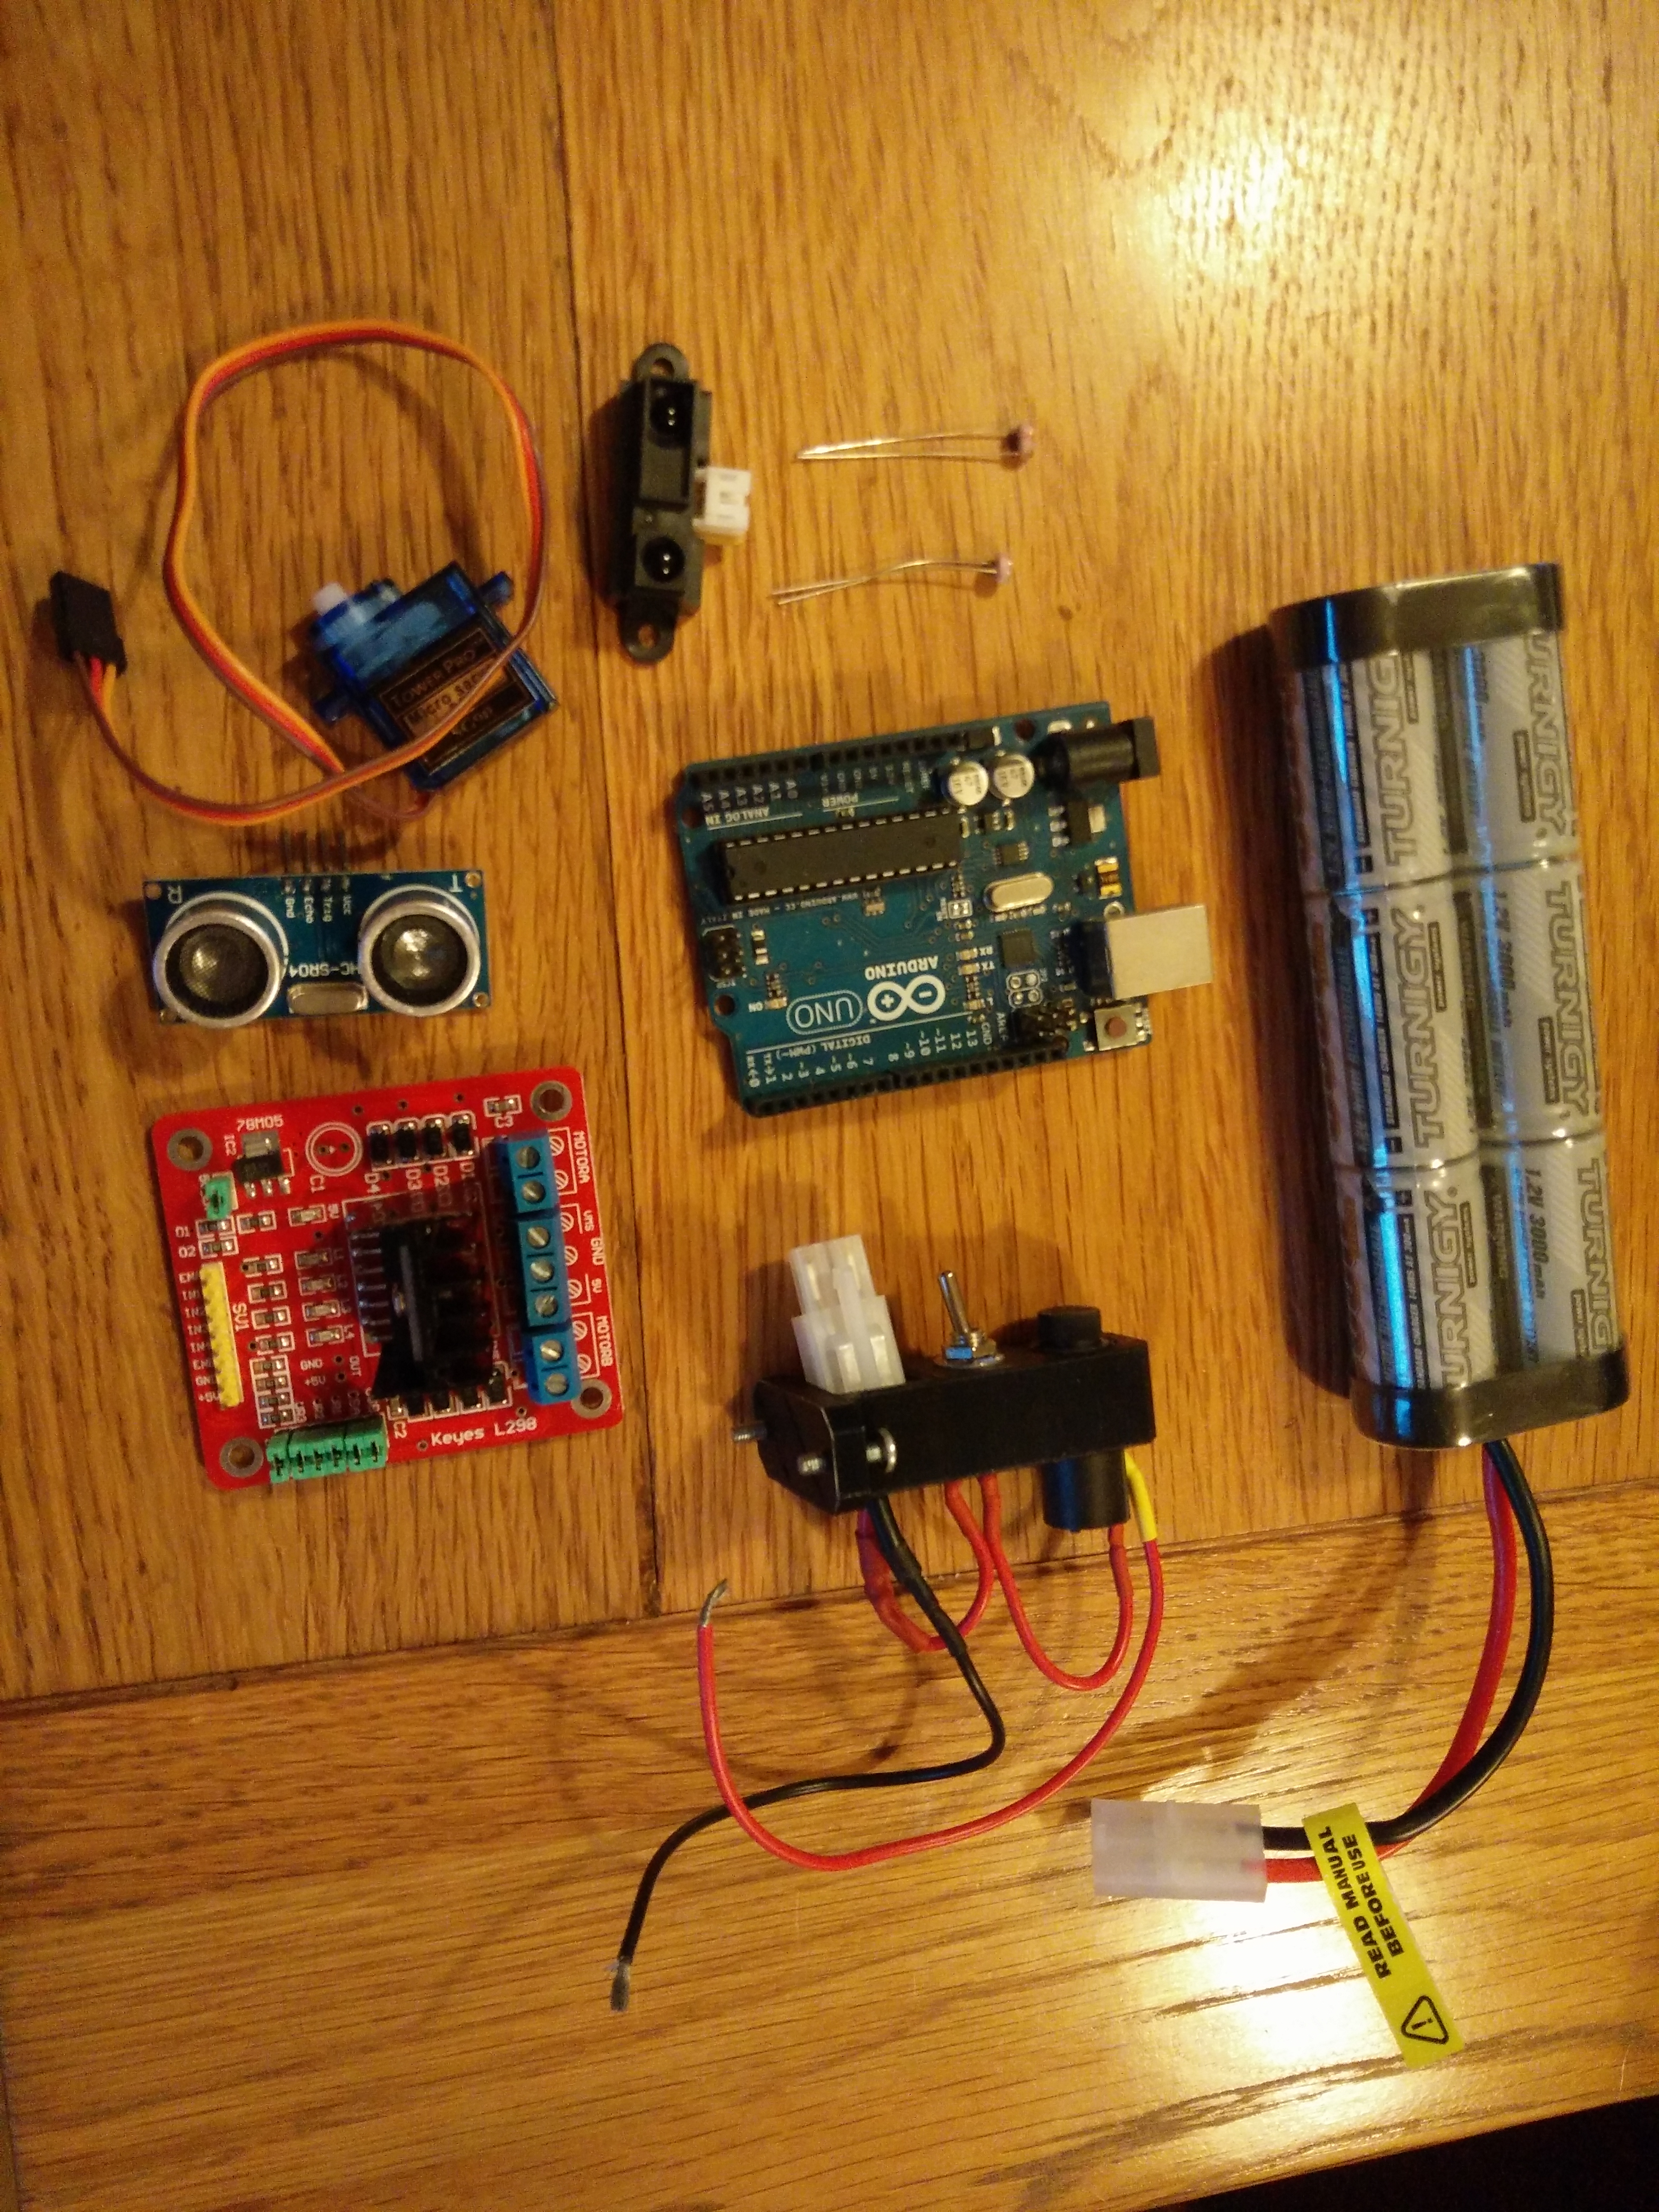
\includegraphics[width=0.6\linewidth, angle=90]{img/content.jpg}
	\end{center}
    
    \cy{Mae'r testun hwn yn Gymraeg.}
    \en{This includes:}
    
    \begin{itemize}
    
    \item{
    \cy{Mae'r testun hwn yn Gymraeg.}
    \en{Nickel Metal Hydride Battery - 7.4v, 3000mAh}}
    
    \item{
    \cy{Mae'r testun hwn yn Gymraeg.}
    \en{Motor Controller - H-Bridge}}
    
    \item{
    \cy{Mae'r testun hwn yn Gymraeg.}
    \en{Fuse and connector holder}}
    
    \item{
    \cy{Mae'r testun hwn yn Gymraeg.}
    \en{Servo Motor}}
    
    \item{
    \cy{Mae'r testun hwn yn Gymraeg.}
    \en{Ultrasonic}}
    
    \item{
    \cy{Mae'r testun hwn yn Gymraeg.}
    \en{Infrared}}
    
    \item{
    \cy{Mae'r testun hwn yn Gymraeg.}
    \en{LDR x2}}
    
    \end{itemize}
    
    \cy{Mae'r testun hwn yn Gymraeg.}
    \en{Some hardware will be handed out when required (just to keep you and the hardware safe).}
    
    \newpage
    
    \section*{%
    \cy{Shwmae!}
    \en{Control Systems}}
    
    \begin{enumerate} %Begin numbered instructions for this section
    
    \item{
    \cy{Mae'r testun hwn yn Gymraeg.}
    \en{\textbf{Oull the motor cables through the pre-defined holes in the chassis.}}
    
    \cy{Mae'r testun hwn yn Gymraeg.}
    \en{This will allow us to plug it into the motor controller.}
    
    \cy{Mae'r testun hwn yn Gymraeg.}
    \en{If there are no cables connected to the motor, you will need to solder the cables to the tags on the motor. Ask a helper if you need a hand with the soldering.}
    
    \begin{center}
    \includegraphics[width=0.7\linewidth]{img/1.jpg}
    \end{center}}
    
    \item{
    \cy{Mae'r testun hwn yn Gymraeg.}
    \en{\textbf{Position the motor controller in an area where the cables from the motors can comfortably reach the controller.}}
    
    \begin{center}
    \includegraphics[width=0.7\linewidth]{img/2.jpg}
    \end{center}}
    
    \newpage
    
    \item{
    \cy{Mae'r testun hwn yn Gymraeg.}
    \en{\textbf{Connect the motors to the motor controller.}}
    
    \cy{Mae'r testun hwn yn Gymraeg.}
    \en{In the picture below it has been wired in the following way.}
    
    \begin{center}
    \begin{tabular}{|p{4cm}|p{4cm}|}
     \hline
     \cy{Mae'r testun hwn yn Gymraeg.}
     \en{Motor Cable & Motor Controller Pin}\\
     \hline
     \cy{Mae'r testun hwn yn Gymraeg.}
     \en{Left Motor - Red & OUT1} \\
     \hline
     \cy{Mae'r testun hwn yn Gymraeg.}
     \en{Left Motor - Black & OUT2}\\
      \hline
     \cy{Mae'r testun hwn yn Gymraeg.}
     \en{Right Motor - Red & OUT3}\\
     \hline
      \cy{Mae'r testun hwn yn Gymraeg.}
     \en{Right Motor - Black & OUT4}\\
      \hline
    \end{tabular}
    \end{center}

    \begin{center}
    \includegraphics[width=0.7\linewidth]{img/3.jpg}
    \end{center}

    \cy{Mae'r testun hwn yn Gymraeg.}
    \en{These cables are outputting power from the motor controller to the motors to make them move.}}
    
    \newpage
    
    \item{
    \cy{Mae'r testun hwn yn Gymraeg.}
    \en{\textbf{Position the Arduino.}}
    
    \cy{Mae'r testun hwn yn Gymraeg.}
    \en{We now need to add the brains to our robot. As we will be connecting the Arduino to the motor
controller to send signals, the motor controller and the Arduino will need to be close together.}

    \cy{Mae'r testun hwn yn Gymraeg.}
    \en{To raise the Arduino off the plastic we use the golden spacers.}
    
    \cy{Mae'r testun hwn yn Gymraeg.}
    \en{Ensure that the USB port is accessible so you can programme the Arduino later on.}
    
    \begin{center}
    \includegraphics[width=0.7\linewidth]{img/4.jpg}\par
    \includegraphics[width=0.7\linewidth]{img/5.jpg}
    \end{center}}
    
    \newpage
    
    \item{
    \cy{Mae'r testun hwn yn Gymraeg.}
    \en{\textbf{Connect cables to the motor controllers}}
    
    \cy{Mae'r testun hwn yn Gymraeg.}
    \en{There are 4 pins sticking out of the motor controller, each one represents a cable on the motor.}
    
    \begin{center}
    \includegraphics[width=0.7\linewidth]{img/6.jpg}
    \end{center}
    
    \cy{Mae'r testun hwn yn Gymraeg.}
    \en{You will now need 4 new cables.}
    
    \cy{Mae'r testun hwn yn Gymraeg.}
    \en{Using the female-to-male jumper cables, connect the cables from left to right as seen in the
picture above.}
    
    \cy{Mae'r testun hwn yn Gymraeg.}
    \en{An example of these cables can be found in the picture below:}
    
    \begin{center}
    \includegraphics[width=0.7\linewidth]{img/7.jpg}
    \end{center}}
    
    \newpage
    
    \item{
    \cy{Mae'r testun hwn yn Gymraeg.}
    \en{\textbf{Starting from left to right on the motor controller, connect this up to the Arduino.}}
    
    \cy{Mae'r testun hwn yn Gymraeg.}
    \en{Below is the digital pin latout for an Arduino Uno.}
    
    \begin{center}
    \begin{tabular}{|p{4cm}|p{4cm}|}
     \hline
     Motor Controller & Arduino Pin\\
     \hline
     Motor Controller 1 & Arduino \textasciitilde 5\\
     \hline
     Motor Controller 2 & Arduino \textasciitilde 6\\
     \hline
     Motor Controller 3 & Arduino \textasciitilde 9\\
     \hline
      Motor Controller 4 & Arduino \textasciitilde 10\\
     \hline
    \end{tabular}
    \end{center}
    
    \begin{center}
    \includegraphics[width=0.7\linewidth]{img/8.jpg}\par
    \includegraphics[width=0.7\linewidth]{img/9.jpg}
    \end{center}}
    
    \newpage
    
    \item{
    \cy{Mae'r testun hwn yn Gymraeg.}
    \en{\textbf{Connect the red cable from the power block into the VIN plug.}}
    
    \cy{Mae'r testun hwn yn Gymraeg.}
    \en{The blue sockets on the motor controller are labelled VIN, GND and +5V. This step will supply 7.4 volts from the battery into the motor controller.}
    
    \cy{Mae'r testun hwn yn Gymraeg.}
    \en{The power block acts as the gateway between the battery and the motor controller. This includes a connector to remove the battery, a switch to turn the robot on and off, and a fuse to ensure the battery and circuit remains safe.}
    
    \begin{center}
    \includegraphics[width=0.7\linewidth]{img/10.jpg}
    \end{center}}
    
    \item{
    \cy{Mae'r testun hwn yn Gymraeg.}
    \en{\textbf{Connect the black cable from the power block into the GND plug.}}
    
    \cy{Mae'r testun hwn yn Gymraeg.}
    \en{This will act as ground from the battery.}
    
    \begin{center}
    \includegraphics[width=0.7\linewidth]{img/11.jpg}
    \end{center}}
    
    \item{
    \cy{Mae'r testun hwn yn Gymraeg.}
    \en{\textbf{Secure the power block to the chassis.}}
    
    \cy{Mae'r testun hwn yn Gymraeg.}
    \en{This is to prevent the electronics from moving around whilst the robot is driving.}
    
    \begin{center}
    \includegraphics[width=0.7\linewidth]{img/12.jpg}
    \end{center}}
    
    \item{
    \cy{Mae'r testun hwn yn Gymraeg.}
    \en{\textbf{Use a custom jumper cable to connect pins ENA, ENB and +5v on the motor controller.}}
    
    \cy{Mae'r testun hwn yn Gymraeg.}
    \en{These red motor controllers have pins which allow you to turn the power to enable the motors
to be used. ENA and ENB. We want these to be connected to 5v as we want to be able to use
the motors anytime we want.}
    
    \begin{center}
    \includegraphics[width=0.7\linewidth]{img/16.jpg}
    \end{center}}
    
    \newpage
    
    \item{
    \cy{Mae'r testun hwn yn Gymraeg.}
    \en{\textbf{Connect a male-to-male jumper cable into the 5V pin on the motor controller and add it to VIN on the Arduino.}}
    
    \cy{Mae'r testun hwn yn Gymraeg.}
    \en{We need to send power to the Arduino, we can use the same battery as the motor controller by piggy-backing off the motor controller regulator that turns 7.4 volts to 5 volts.}}
    
    \item{
    \cy{Mae'r testun hwn yn Gymraeg.}
    \en{\textbf{Connect a male-to-male jumper cable into the GND pin on the motor controller and add it to GND on the Arduino.}}
    
    \cy{Mae'r testun hwn yn Gymraeg.}
    \en{See the picture below to see how to power.}
    
    \begin{center}
    \includegraphics[width=0.7\linewidth]{img/13.jpg}\par
    \includegraphics[width=0.7\linewidth]{img/14.jpg}
    \end{center}}
    
    \newpage
    
    \item{
    \cy{Mae'r testun hwn yn Gymraeg.}
    \en{\textbf{Call a helper to let them know you are finished and need a battery.}}
    
    \cy{Mae'r testun hwn yn Gymraeg.}
    \en{Once you have finished all the previous steps, you are ready to add the battery. A helper will check your circuit to make sure it is safe to add the battery.}
    
    \begin{center}
    \includegraphics[width=0.7\linewidth]{img/15.jpg}\par
    \includegraphics[width=0.7\linewidth]{img/12.jpg}
    \end{center}}
    
    \end{enumerate}
    
    \cy{Mae'r testun hwn yn Gymraeg.}
    \en{You are now ready to move along to the programming worksheet to test your drive systems.}

    \end{document}